\documentclass{article}
\usepackage{geometry}
\geometry{
	a4paper,
	left=2.5cm,
	right=2.5cm,
	top=2.5cm,
	bottom=2.5cm,
	headheight=13.6pt
}
% 最简单、最稳定的中文方案（自动适配系统，永不报错）
\usepackage[UTF8, scheme=plain]{ctex}
% 设置英文默认字体为 Times New Roman
\usepackage{fontspec}
\setmainfont{Times New Roman}
\usepackage{amsmath}
\usepackage{amssymb}
\usepackage{booktabs}
\usepackage{caption}
\usepackage{setspace}
\doublespacing
\setlength{\parskip}{4pt}
\usepackage{array}
\usepackage{listings}
\usepackage{graphicx}
\usepackage{enumitem}
\usepackage{subcaption}
\usepackage{multirow}
\usepackage{mathrsfs}
\usepackage{bm}
\usepackage{xcolor}
\usepackage{colortbl}
\usepackage{tikz}
\usepackage{tikz-3dplot}
\usetikzlibrary{
	arrows.meta,
	calc,
	patterns,
	decorations.pathmorphing,
	backgrounds,
	positioning,
	fit,
	shapes.geometric,
	intersections,
	through,
	angles,
	quotes,
	plotmarks
}
%目录超链接
\usepackage{hyperref}
\hypersetup{
	colorlinks=true,
	linkcolor=black,
	filecolor=magenta,
	urlcolor=cyan,
}
\usepackage{tocloft}
\setlength{\cftbeforesecskip}{2ex}
\setlength{\cftbeforesubsecskip}{1ex}
\setlength{\cftbeforesubsubsecskip}{1ex}
% 定义代码颜色
\definecolor{codegreen}{rgb}{0,0.6,0}
\definecolor{NavyBlue}{RGB}{0,0,128}
\definecolor{PineGreen}{RGB}{1,121,111}
% 配置 listings 环境
\lstset{
	language=TeX,
	tabsize=4,
	captionpos=b,
	numbers=left,
	numbersep=1em,
	sensitive=true,
	showtabs=false,
	frame=shadowbox,
	breaklines=true,
	keepspaces=true,
	showspaces=false,
	showstringspaces=false,
	breakatwhitespace=false,
	basicstyle=\ttfamily\normalsize,
	keywordstyle=\color{NavyBlue},
	commentstyle=\color{codegreen},
	numberstyle=\color{black},
	stringstyle=\color{PineGreen!90!black},
	rulesepcolor=\color{red!20!green!20!blue!20},
	escapeinside={/@}{@/},
}
% 自定义颜色
\definecolor{LightGreen}{rgb}{0.9, 0.95, 0.9}
\definecolor{LightBlue}{RGB}{229, 238, 255}
\definecolor{LightPink}{RGB}{255, 229, 237}
\definecolor{DarkRed}{RGB}{169,0,0}
\definecolor{DarkGreen}{RGB}{0,110,12}
\definecolor{SkyBlue}{RGB}{0,114,255}
% 自定义环境 无缩进
\newenvironment{knowledge}[1]{%
	\noindent{%
		\normalfont\bfseries\color{DarkRed} #1}\hskip 0.5em%
	\color{DarkRed}%
}{%
	\par\color{black}%
}
\newenvironment{question}[1][]{%
	\noindent
	\ifx\relax#1\relax\else
	{%
		\normalfont\color{DarkGreen} #1}\hskip 0.5em%
	\fi
	\color{DarkGreen}%
}{%
	\ifhmode\fi\color{black}%
}
\newcommand{\category}[1]{%
	\noindent{%
		\normalfont\bfseries\color{SkyBlue} #1}\hskip 0.5em}
\captionsetup[table]{
	justification=centering,
	labelsep=quad,
	font={bf}
}
\captionsetup[figure]{
	justification=centering,
	labelsep=quad,
	font={bf}
}
\captionsetup[subfigure]{
	font={bf}
}
\begin{document}
	
	\begin{center}
		
		{\LARGE \textbf{数理统计笔记}} \\[0.5cm]
		{\large {\kaishu 石继楷 \quad 编写}} \\[0.3cm]
		{\normalsize 2026年9月16日}
	\end{center}
	\tableofcontents
	\newpage
	
	\section{第五章\quad 统计量及其分布}
	\subsection{§5.1\quad 总体与样本}
	\begin{knowledge}{总体、个体与样本}
		
		总体：研究对象的全体.
		
		个体：总体的每个成员.
		
		样本：从总体中抽取 $X_1, \dots, X_n$，每一个称为样本点.
		
		样本容量：$n$.
		
		完全样本：每一个具体数值均已知.
		
		不完全样本：信息缺失（值 $\to$ 区间）.
	\end{knowledge}
	
	\begin{knowledge}{随机抽样的要求}
		
		代表性：同等机会被选入样本.
		
		独立性：抽样不影响取值.
		
		上述两条要求即 $X_1,\dots,X_n$ 独立同分布，记作 i.i.d.
	\end{knowledge}
	
	\subsection{§5.2\quad 样本数据的整理与显示}
	\begin{knowledge}{经验分布函数}
		
		设样本观测值为 $x_1,\dots,x_n$，排序后为 $x_{(1)} \leq \dots \leq x_{(n)}$，则经验分布函数为
		\[
		F_n(x) =
		\begin{cases}
			0, & x < x_{(1)}, \\[4pt]
			\dfrac{k}{n}, & x_{(k)} \leq x < x_{(k+1)},\quad k=1,2,\dots,n-1, \\[4pt]
			1, & x \geq x_{(n)}.
		\end{cases}
		\]
		或记
		\[
		I_i(x) =
		\begin{cases}
			1, & x_i \leq x, \\
			0, & x_i > x,
		\end{cases}
		\]
		则
		\[
		F_n(x) = \frac{1}{n} \sum_{i=1}^n I_i(x).
		\]
	\end{knowledge}
	
	\begin{minipage}[t]{0.7\textwidth}
		
		\begin{knowledge}{频率分布表与直方图}
			
			频率分布表各列：组序、分组区间、组中值、频数、频率、累计频率（累计）.
			
			直方图以分组区间为横轴、以频数（或频率/组距）为纵轴，每个矩形的宽为组距、高为频数，用以直观显示样本数据的分布.
		\end{knowledge}
	\end{minipage}
	\hfill
	\begin{minipage}[t]{0.3\textwidth}
		
		\centering
		\begin{tikzpicture}[scale=0.8, baseline=(current bounding box.north)]
			\draw[->, gray!40] (-0.3,0) -- (4.6,0) node[right] {$x$};
			\draw[->, gray!40] (0,-0.2) -- (0,2.6) node[above] {频数};
			\draw[thick, DarkRed] (0.4,0) rectangle (1.2,1.1);
			\draw[thick, DarkRed] (1.2,0) rectangle (2.0,2.1);
			\draw[thick, DarkRed] (2.0,0) rectangle (2.8,0.9);
			\draw[thick, DarkRed] (2.8,0) rectangle (3.6,0.4);
			\foreach \t in {0.4,1.2,2.0,2.8,3.6}
			\draw (\t,0.06) -- (\t,-0.06);
		\end{tikzpicture}
	\end{minipage}
	
	\subsection{§5.3\quad 统计量及其分布}
	\begin{knowledge}{统计量与抽样分布}
		
		设 $X_1,\dots,X_n$ 为样本，$T(X_1,\dots,X_n)$（不含未知参数）为统计量，其分布称为抽样分布.
	\end{knowledge}
	
	\begin{knowledge}{定理（样本均值的精确分布）}
		
		若总体分布为 $N(\mu, \sigma^2)$，则 $\bar{X}$ 的精确分布为
		\[
		\bar{X} \sim N\left(\mu, \frac{\sigma^2}{n}\right).
		\]
	\end{knowledge}
	
	\begin{knowledge}{样本矩、偏度与峰度}
		
		$k$ 阶原点矩：$a_k = \dfrac{1}{n} \displaystyle\sum_{i=1}^n X_i^k$.
		
		$k$ 阶中心矩：$b_k = \dfrac{1}{n} \displaystyle\sum_{i=1}^n (X_i - \bar{X})^k$.
		
		样本偏度：$\hat{\beta}_S = \dfrac{b_3}{b_2^{3/2}}$.
		
		样本峰度：$\hat{\beta}_K = \dfrac{b_4}{b_2^2} - 3$.
	\end{knowledge}
	
	\begin{knowledge}{次序统计量}
		
		排序后得到的第 $i$ 个观测值记为 $X_{(i)}$.
		
		$X_{(1)}$ 为最小次序统计量；$X_{(n)}$ 为最大次序统计量.
		
		$(X_{(1)}, \dots, X_{(n)})$ 称为样本次序统计量.
	\end{knowledge}
	
	\begin{knowledge}{单个次序统计量的分布}
		
		设总体密度函数为 $p(x)$，分布函数为 $F(x)$，则 $X_{(k)}$ 的密度函数为
		\[
		p_k(x) = \frac{n!}{(k-1)!\,(n-k)!} \left[F(x)\right]^{k-1} \left[1-F(x)\right]^{n-k} p(x).
		\]
		离散型：
		\[
		P(X_{(k)} \leq m) = \sum_{j=k}^n C_n^j \left[F(m)\right]^j \left[1-F(m)\right]^{n-j},
		\]
		特别地，
		\[
		P(X_{(n)} \leq m) = \left[F(m)\right]^n, \quad P(X_{(n)} = m) = \left[F(m)\right]^n - \left[F(m^-)\right]^n,
		\]
		\[
		P(X_{(1)} = m) = \left[1-F(m^-)\right]^n - \left[1-F(m)\right]^n.
		\]
	\end{knowledge}
	
	\begin{knowledge}{中位数与 $p$ 分位数}
		
		中位数：
		\[
		m_{0.5} =
		\begin{cases}
			X_{\left(\frac{n+1}{2}\right)}, & n \text{ 为奇数}, \\[8pt]
			\dfrac{1}{2}\left(X_{\left(\frac{n}{2}\right)} + X_{\left(\frac{n}{2}+1\right)}\right), & n \text{ 为偶数}.
		\end{cases}
		\]
		$p$ 分位数（$0<p<1$）：
		\[
		m_p =
		\begin{cases}
			X_{([np]+1)}, & np \text{ 不是整数}, \\[6pt]
			\dfrac{1}{2}\left(X_{(np)} + X_{(np+1)}\right), & np \text{ 是整数},
		\end{cases}
		\]
		其中 $[\cdot]$ 取整数部分；$np$ 不是整数时取 $[np]+1$，即向上取整.
	\end{knowledge}
	
	\begin{knowledge}{定理（$p$ 分位数的渐近分布）}
		
		\[
		m_p \sim N\left(x_p,\ \frac{p(1-p)}{n \cdot p^2(x_p)}\right),
		\]
		其中 $x_p$ 为总体的 $p$ 分位数，$p(\cdot)$ 为总体密度函数. 特别地，中位数：
		\[
		m_{0.5} \sim N\left(x_{0.5},\ \frac{1}{4n \cdot p^2(x_{0.5})}\right).
		\]
	\end{knowledge}
	
	\subsection{五数概括与箱线图}
	\begin{minipage}[t]{0.7\textwidth}
		
		\begin{knowledge}{五数概括}
			
			下列五个数
			\[
			X_{(1)},\quad m_{0.25},\quad m_{0.5},\quad m_{0.75},\quad X_{(n)},
			\]
			即
			\[
			X_{\min},\quad Q_1,\quad m_{0.5}\ (Q_2),\quad Q_3,\quad X_{\max},
			\]
			称为五数概括.
		\end{knowledge}
		
		\begin{knowledge}{箱线图}
			
			箱体自 $Q_1$ 画到 $Q_3$，箱内竖线为中位数 $m_{0.5}$；两侧须分别延伸至 $X_{\min}$ 与 $X_{\max}$. 箱线图可快速读出数据的中心、散布与对称性.
		\end{knowledge}
	\end{minipage}
	\hfill
	\begin{minipage}[t]{0.3\textwidth}
		
		\centering
		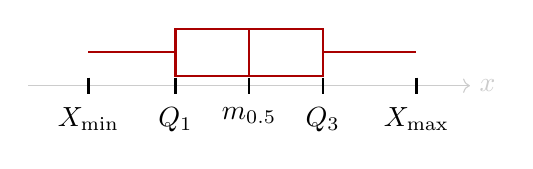
\begin{tikzpicture}[scale=0.85, baseline=(current bounding box.north)]
			\draw[->, gray!40] (-0.4,0) -- (6.2,0) node[right] {$x$};
			\foreach \t in {0.5,1.8,2.9,4.0,5.4}
			\draw[thick] (\t,0.12) -- (\t,-0.12);
			\draw[thick, DarkRed] (0.5,0.5) -- (1.8,0.5);
			\draw[thick, DarkRed] (4.0,0.5) -- (5.4,0.5);
			\draw[thick, DarkRed] (1.8,0.15) rectangle (4.0,0.85);
			\draw[thick, DarkRed] (2.9,0.15) -- (2.9,0.85);
			\node[below] at (0.5,-0.18) {$X_{\min}$};
			\node[below] at (1.8,-0.18) {$Q_1$};
			\node[below] at (2.9,-0.18) {$m_{0.5}$};
			\node[below] at (4.0,-0.18) {$Q_3$};
			\node[below] at (5.4,-0.18) {$X_{\max}$};
		\end{tikzpicture}
	\end{minipage}
	
\end{document}